\section{Technologies}
Building Fidelis required collating a number of technologies. The technologies used for implementation can be categorised into storage, processing and visualisation technologies, each of which are discussed below.

\subsection{Storage}
MySQL is an open source database management system used for managing data held in a relational database management system \cite{MySQL:Home}. It is the world's most popular open source database, being used by some of the largest and fastest-growing organisations including Facebook, Google and Adobe. The reasons behind the use of MySQL database are vast but the key factor is the ease with which a MySQL database can be setup and migrated. MySQL databases have existed for many years which has led to gradual improvements over time, and as a result of these improvements MySQL databases now guarantee stability, scalability and security \cite{MySQL:Why}. The longevity of MySQL database systems is another appealing aspect, and has meant that a wide range of third-party party tools are available to the developer for working with and processing the data. 

\subsection{Processing}
Majority of the data processing will be done using PHP. All PHP scripts are executed on the server which may produce output that can be presented to the user. The language is used by millions of websites and has for some time been  a popular scripting language for dynamic web development. This wide adoption of the PHP scripting language has allowed extensive libraries and frameworks to be made available and used for rapid development of web applications. One such framework, Laravel, will be used to implement the MVC approach discussed in Chapter \ref{Chapter:Research}. PHP has shown to be scalable as it is powerful enough to be at the core of the biggest blogging system on the web, known as WordPress, but at the same time it is deep enough to run the largest social network, Facebook\cite{W3Schools:PHP_Intro, Wiki:WordPress, Fastcompany:Facebook_PHP}. This means that in the future if the system is to grow large enough, it can easily be scaled as done so over time by the aforementioned examples. 

In addition to PHP, JavaScript will be used for some client-side data processing along with SQL which will be used to process data from the database before it is retrieved. Python will be used to process user data needed for content-filtering, abuse detection, recommendations and reputation scoring. Like PHP, Python is also executed on the server-side, reducing the amount of processing and computation required on the client-side. Python was chosen not only for its popularity, but again like PHP it provides an extensive range of libraries that can be used during development. Examples of these include Scikit-Learn \cite{scikit:home}, which provides a number of data mining and analysis tools, and \emph{NumPy} and \emph{pandas}, which are useful for data manipulation.

It was mentioned in Chapter \ref{Chapter:Design} that it would not be feasible to run the data processing algorithms in real-time, and as such these would need to be scheduled to run at set intervals. Cron is a unix- system utility that is used to execute tasks at designated times \cite{Ubuntu:Cron}. Tasks that are scheduled for execution are contained in a \textit{crontab} file. Entries in the file appear as:
\begin{lstlisting}[language=bash]
* * * * * command/to/run
\end{lstlisting}

Each asterix represents a time-and-date field, and from left to right these correspond to minute, hour, day, month and weekday \cite{Ubuntu:Cron}. 

Laravel contains a task scheduler which simplifies the process of executing tasks at a given interval. With the scheduler, only the following entry needs to be added to the \textit{crontab} file:

\begin{lstlisting}[language=bash]
* * * * * php /path-to-your-project/artisan schedule:run >> /dev/null 2>&1
\end{lstlisting}

This entry calls the Laravel task scheduler every minute \cite{Laravel:Scheduling}. Laravel's task scheduler provides a number of schedule frequency options, including daily, weekly or even as a custom cron entry \cite{Laravel:Scheduling}. Tasks can be added to the \texttt{schedule()} method in \textit{app/Console/Kernel}. In the method, it is possible to schedule Artisan commands, which can be made by the user, or OS commands. Custom user commands can be defined using the following command:

\begin{lstlisting}[language=bash]
php artisan make:command CommandName --command=commandsignature
\end{lstlisting}

When this command is run, it created a command class whereby a custom command can be defined in the \texttt{handle()} function. Figure \ref{fig:FidelisSchedule} shows the tasks scheduled to run daily at midnight, and one task set to run weekly.

\begin{figure}[H]
\centering
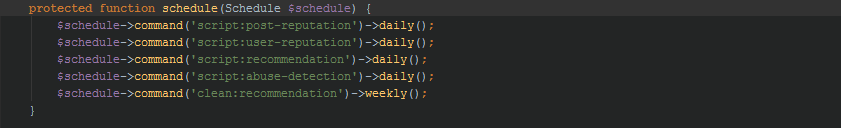
\includegraphics[width=\textwidth]{Images/Implementation/FidelisSchedule}
\caption{Scheduled tasks for Fidelis}
\label{fig:FidelisSchedule}
\end{figure}

\subsection{Visualisation}
HTML is coupled with CSS to define page structure, and design the components on the page \cite{W3:HTML5, W3:CSS}. In addition to this, the Laravel blade engine is being used to make the generation of pages easier by splitting content up into views that can be extended by or rendered inside other views \cite{Laravel:Blade}. This encourages good practices by abstracting the system and enforcing modularity throughout. Using the blade enginge supported the idea of using component-driven design, discussed in Chapter \ref{Chapter:ProjectManagement}. Building views in a modular fashion enables development in the future to easily integrate new components and replace master views seamlessly to change the overall system appearance. Bootstrap is also used as an additional framework to make the pages more dynamic by providing visual interaction.

\subsection{Installation and Setup}
Many of the technologies being employed are not included by default on an ordinary machine. Thus, before development could be initiated, it was necessary to install and configure the required technologies. This section details the configuration process for the technologies used, along with any prerequisites for them.

\subsubsection{Initial Setup}
An Apache web server capable of interpreting PHP and rendering web pages was required for development. In addition to this, an SQL server was need to host the MySQL database. XAMPP, which provides an SQL and web server, was the solution chosen to handle both these cases. Both servers are automatically configured by the XAMPP package upon installation and are immediately ready to use out of the box. XAMPP provides an easy-to-use control panel from which servers can be started, and accessing through \textit{http://localhost/}. Any files can them be placed inside the \textit{htdocs} folder, created during the installation process.

\subsubsection{IDE and Laravel}
The Laravel framework was used to build Fidelis, but it is not readily available to download as an archive. Instead, composer - a package manager, was used for the installation of the framework. Using composer, new projects can be created using the \textit{laraval new project-name} command. Executing this command creates a new \textit{project-name} directory with all the necessary files and project dependencies. Updates and additional packages may be installed using composer and the included \textit{packages.json} file.

The PHPStorm IDE, developed by JetBrains, was used throughout the project for all web-related development. PHPStorm is a dedicated PHP IDE, and has the capability to include plugins providing features that enable the use of frameworks like Laravel. The IDE also makes available a set of tools that made writing code more efficient and effective.